\subsection{Tổng hợp tin nhắn tạo lịch trình}

Một trong những tính năng ứng dụng AI nổi bật của VieVu là khả năng phân tích nội dung hội thoại trong nhóm chat và tự động đề xuất bản nháp lịch trình chi tiết cho chuyến đi. Để hiện thực hóa tính năng này một cách hiệu quả, tránh việc phải xử lý lại toàn bộ lịch sử trò chuyện mỗi khi người dùng yêu cầu, một kiến trúc xử lý gồm hai giai đoạn chính đã được thiết kế và triển khai trên nền tảng server FastAPI:

\subsubsection{Giai đoạn 1: Tiền xử lý Tin nhắn Bất đồng bộ}
\label{subsubsec:summary_phase1}

Giai đoạn đầu tiên của pipeline tập trung vào việc xử lý các tin nhắn mới ngay khi chúng được gửi đến hệ thống, nhằm mục đích phân loại và trích xuất thông tin liên quan một cách tự động và bất đồng bộ.
\begin{enumerate}
    \item  \textbf{Lắng nghe sự kiện Tin nhắn Mới}

 Để phát hiện tin nhắn mới một cách hiệu quả, hệ thống sử dụng cơ chế \textbf{LISTEN/NOTIFY} tích hợp sẵn của PostgreSQL. Một trigger cơ sở dữ liệu được cấu hình trên bảng \texttt{messages} để mỗi khi có một bản ghi mới được chèn, nó sẽ gửi một thông báo đến một kênh được tạo là \texttt{messages\_insert}, kèm theo dữ liệu (payload) của tin nhắn mới dưới dạng JSON (xem ví dụ tại Đoạn mã~\ref{lst:json-payload}). % (Xem chi tiết trigger tại Phụ lục \ref{apdx:db_trigger}) % <<< Placeholder
 \newpage
 \lstset{language=json}
\begin{lstlisting}[
    caption=Payload JSON của tin nhắn mới (dạng dictionary Python),
    label=lst:json-payload,
    captionpos=t,
    belowcaptionskip=10pt,
    basicstyle=\small\ttfamily,
    breaklines=true,
    showstringspaces=false,
    inputencoding=utf8] 
{
    'id': 335,
    'created_at': '2025-04-23T03:54:26.25777+00:00',
    'content': 'Thu den Vinh Ha Long xem the nao cung duoc',
    'chat_id': 1,
    'meta_data': None,
    'is_travel_related': None,
    'chat_member_id': 10
}
\end{lstlisting}

Phía server FastAPI, một tác vụ nền \texttt{listen\_to\_messages} sử dụng thư viện \texttt{asyncio} của Python được khởi chạy và duy trì hoạt động liên tục nhờ cơ chế quản lý vòng đời \texttt{lifespan} của FastAPI. Tác vụ này thực hiện lệnh \texttt{LISTEN messages\_insert;} để lắng nghe các thông báo được gửi từ PostgreSQL trên kênh đã định. % (Xem mã nguồn hàm lắng nghe tại Đoạn mã \ref{lst:listener_code}) % <<< Placeholder

\item  \textbf{Xử lý dữ liệu tin nhắn}

\noindent Khi tác vụ nền \texttt{listen\_to\_messages} nhận được một thông báo tin nhắn mới, nó sẽ thực hiện tuần tự các bước xử lý sau đây trên dữ liệu payload nhận được:
\begin{itemize}
    \item \textbf{Phân loại Zero-Shot (ZSC):} Nội dung tin nhắn được đưa vào hàm \texttt{classify\_sentence}, sử dụng mô hình \texttt{joeddav/xlm-roberta-large-xnli} với 2 tag để phân loại là \texttt{"travel schedule information"} và \texttt{"not travel schedule information"}. Kết quả phân loại (ví dụ tại Đoạn mã~\ref{lst:zsc_output}) được dùng để xác định giá trị boolean \texttt{is\_travel\_related} dựa trên điểm tin cậy của nhãn \texttt{"travel schedule information"} $\geq 0.4$.
    \newpage 
    \lstset{language=json}
    \begin{lstlisting}[
        caption=Output phân loại của mô hình ZSC (dạng dictionary Python),
        label=lst:zsc_output,
        captionpos=t,
        belowcaptionskip=10pt,
        basicstyle=\small\ttfamily,
        breaklines=true,
        showstringspaces=false,
        inputencoding=utf8] 
{
    'sequence': 'Thu den Vinh Ha Long xem the nao cung duoc',
    'labels': ['travel schedule information', 'not travel schedule information'],
    'scores': [0.5240467190742493, 0.4759533107280731]
}
    \end{lstlisting}
    \item \textbf{Nhận dạng Thực thể Tên (NER):} Nếu \texttt{is\_travel\_related} là \texttt{true}, nội dung tin nhắn tiếp tục được xử lý bởi hàm \texttt{get\_place\_name} (sử dụng thư viện \texttt{underthesea}). Các thực thể địa điểm (Location) mới được tìm thấy (kết quả ví dụ như trong Đoạn mã~\ref{lst:ner_output}) sẽ được định dạng và bổ sung vào trường \texttt{meta\_data} (JSONB) của tin nhắn, tránh việc lưu trữ trùng lặp thông tin đã có.
    \lstset{language=Python}
    \begin{lstlisting}[
        caption=Output nhận dạng thực thể của thư viện Underthesea,
        label=lst:ner_output, 
        captionpos=t,
        belowcaptionskip=10pt,
        basicstyle=\small\ttfamily,
        breaklines=true,
        showstringspaces=false,
        inputencoding=utf8] 
[
    ('Thu', 'V', 'B-VP', 'O'), 
    ('den', 'E', 'B-PP', 'O'),
    ('Vinh', 'N', 'B-NP', 'B-LOC'),
    ('Ha Long', 'Np', 'I-NP', 'I-LOC'), 
    ('xem', 'V', 'B-VP', 'O'),
    ('the nao', 'P', 'B-NP', 'O'),
    ('cung', 'R', 'O', 'O'),
    ('duoc', 'V', 'B-VP', 'O')
]
    \end{lstlisting}

    \item \textbf{Xử lý Phản hồi Khẳng định/Phủ định:} Áp dụng logic fallback: nếu tin nhắn trước đó liên quan nhưng tin nhắn hiện tại không liên quan (theo ZSC), hàm \texttt{classify\_affirmative} sẽ được gọi để kiểm tra. Hàm này cũng áp dụng mô hình \texttt{joeddav/xlm-roberta-large-xnli} với 2 tag để phân loại là \texttt{"affirmation or negation"} và \texttt{"not affirmation and negation"}. Nếu tin nhắn là lời khẳng định/phủ định \texttt{is\_travel\_related} sẽ được đặt lại thành \texttt{true}.
    \item \textbf{Cập nhật Cơ sở dữ liệu:} Cuối cùng, bản ghi tin nhắn tương ứng trong bảng \texttt{messages} được cập nhật với giá trị \texttt{is\_travel\_related} cuối cùng và trường \texttt{meta\_data} đã được thêm (nếu có).
\end{itemize}
% (Xem chi tiết logic xử lý tại Đoạn mã \ref{lst:message_processing_logic}) % <<< Placeholder

\item  \textbf{Xử lý Dữ liệu Tồn đọng}

\noindent Để đảm bảo không bỏ sót các tin nhắn được gửi trong thời gian server FastAPI không hoạt động, hàm \texttt{update\_travel\_related\_status} được thực thi một lần duy nhất khi server khởi động. Hàm này sẽ truy vấn và thực hiện toàn bộ luồng xử lý ZSC, NER, Affirmation Check như trên cho tất cả các tin nhắn trong cơ sở dữ liệu mà trường \texttt{is\_travel\_related} đang có giá trị NULL.

\end{enumerate}

\noindent Kết thúc Giai đoạn 1, các tin nhắn trong cơ sở dữ liệu đã được phân loại và xử lý thông tin một cách tự động, tạo tiền đề dữ liệu cần thiết và tối ưu cho Giai đoạn 2 - tổng hợp lịch trình theo yêu cầu của người dùng.

\subsubsection{Giai đoạn 2: Tổng hợp và Tạo Lịch trình theo Yêu cầu}
\label{subsubsec:summary_phase2}

Sau khi các tin nhắn đã được tiền xử lý ở Giai đoạn 1, Giai đoạn 2 (hay việc tổng hợp) được kích hoạt chủ động bởi người dùng để tạo ra bản nháp lịch trình cuối cùng. Quá trình này bao gồm các bước xử lý cả ở phía client (Flutter) và server (FastAPI).

\begin{enumerate}
    \item \textbf{Chuẩn bị Dữ liệu Phía Client:}

    Khi người dùng yêu cầu, ứng dụng Flutter truy vấn các tin nhắn liên quan mới nhất từ Supabase (đã được đánh dấu \texttt{is\_travel\_related=true}, mới hơn tin nhắn cuối được tổng hợp) kèm theo thông tin \texttt{message\_reactions}. Ở bước này, Client tự xử lý logic vote từ reaction like hoặc dislike để tạo marker `|Yes|` hoặc `|No|` nối vào cuối nội dung các tin nhắn tương ứng trong input đầu vào. Đồng thời, client thu thập metadata địa điểm, ngày đi và lịch trình cũ (nếu có).


    \item \textbf{Gọi API Tổng hợp Phía Server:} Client Flutter tạo JSON body chứa danh sách \texttt{conversation} (đã xử lý vote), \texttt{metadata}, \texttt{start\_date}, \texttt{end\_date}, và \texttt{previous\_summary} (nếu có), sau đó gửi yêu cầu POST đến endpoint \texttt{/summarize} của server FastAPI cùng token xác thực. Cấu trúc JSON request hoàn chỉnh được minh họa trong Hình~\ref{fig:input}. % (Tham khảo mã gọi API tại Đoạn mã \ref{lst:client_api_call}) % <<< Placeholder
    \begin{figure}[H]
        \centering
        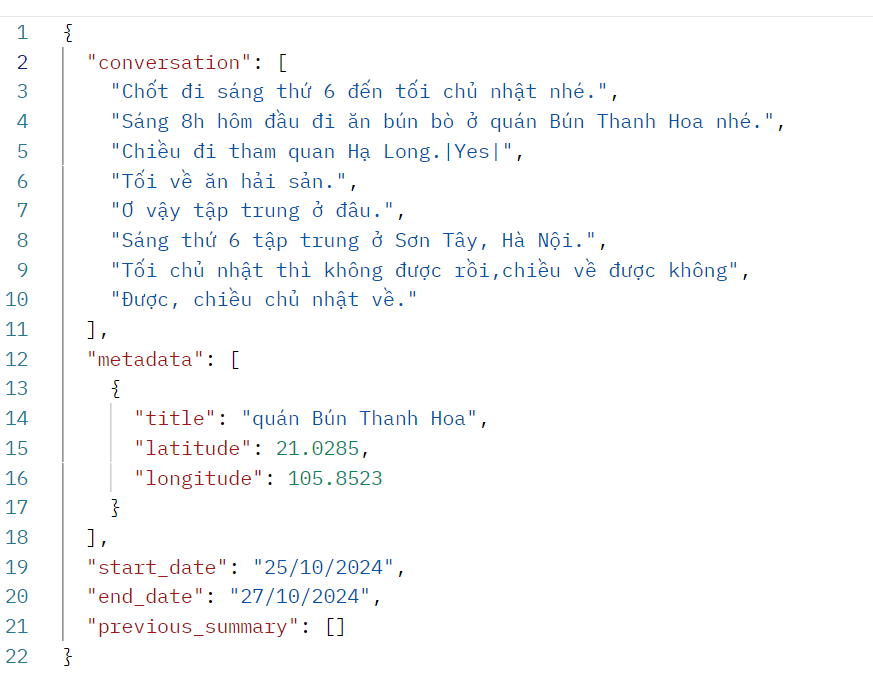
\includegraphics[width=0.8\textwidth]{figures/c4/input.png}
        \caption{JSON request hoàn chỉnh từ client gửi đến server.}
        \label{fig:input}
    \end{figure}
    \item \textbf{Xây dựng Prompt:} Server FastAPI nhận yêu cầu, tổng hợp dữ liệu và xây dựng một prompt chi tiết cho Google Gemini API, như minh họa trong Hình~\ref{fig:prompt}. Prompt này chứa đầy đủ ngữ cảnh và các chỉ dẫn cụ thể về cách tạo lịch trình dạng JSON theo yêu cầu (lọc sự kiện, xử lý Yes/No, liên kết metadata, gộp lịch trình cũ, tuân thủ định dạng outputv.v.). Sau khi prompt hoàn chỉnh, server gửi yêu cầu đến Gemini API. % (Tham khảo cấu trúc prompt chi tiết tại Phụ lục \ref{apdx:gemini_prompt}) % <<< Placeholder
    \begin{figure}[H]
        \centering
        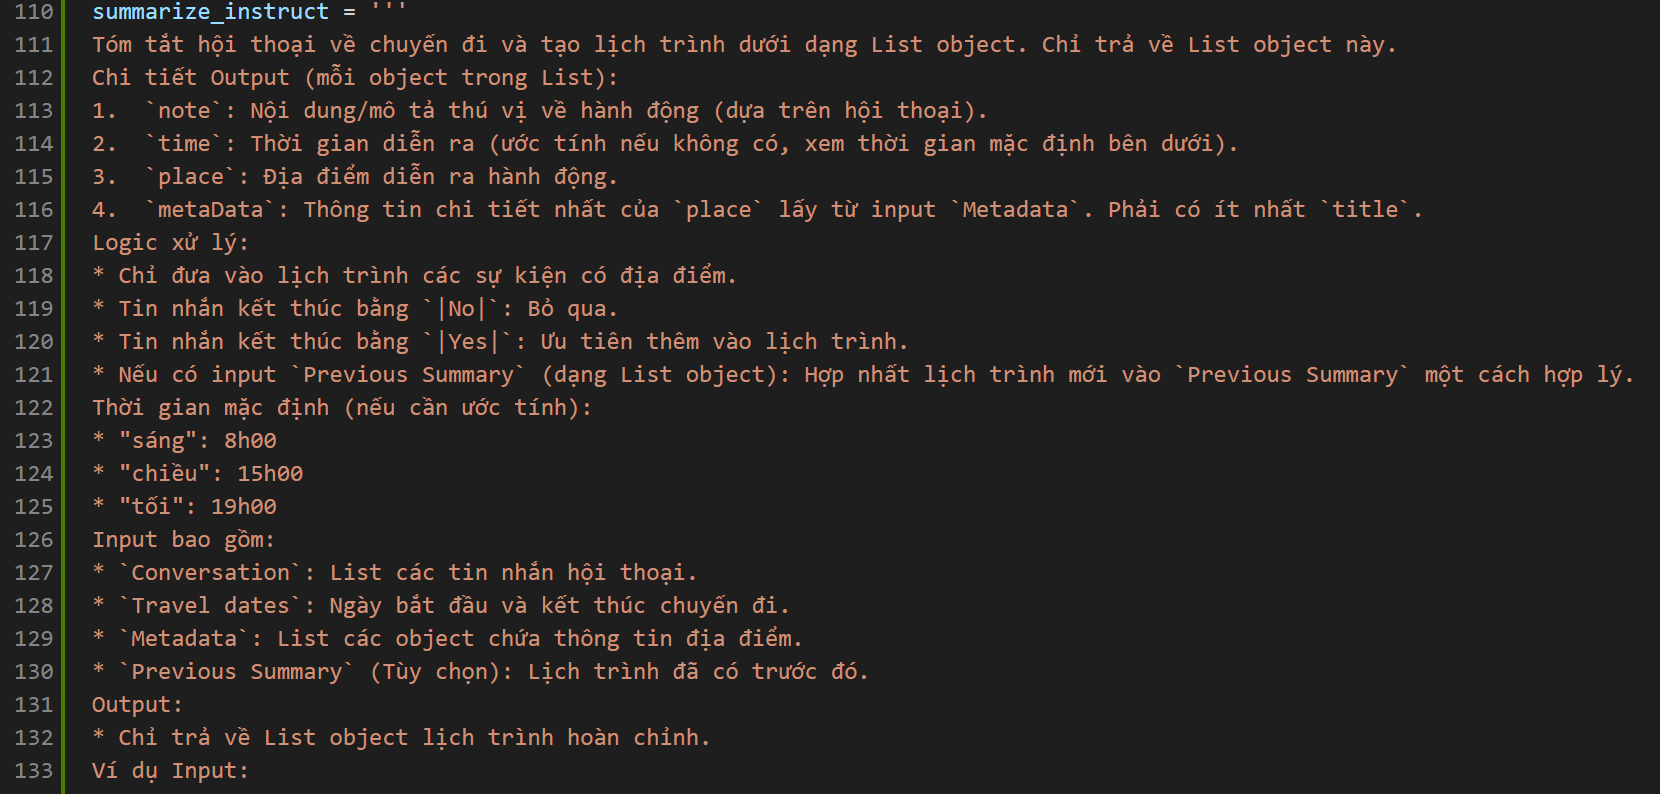
\includegraphics[width=0.8\textwidth]{figures/c4/prompt.png}
        \caption{Prompt hướng dẫn Gemini tổng hợp lịch trình.}
        \label{fig:prompt}
    \end{figure}
    \item \textbf{Xử lý Kết quả, Lưu trữ và Phản hồi:} Server FastAPI nhận phản hồi JSON từ Gemini, phân tích cú pháp để lấy cấu trúc lịch trình. Sau đó, server thực hiện thao tác \texttt{upsert} vào bảng \texttt{chat\_summaries} để lưu/cập nhật lịch trình (\texttt{summary}), bản đọc (\texttt{readings}), và \texttt{last\_message\_id}. Cuối cùng, kết quả lịch trình (ví dụ như trong Hình~\ref{fig:output}) được gửi về client Flutter để hiển thị.
    \begin{figure}[H]
        \centering
        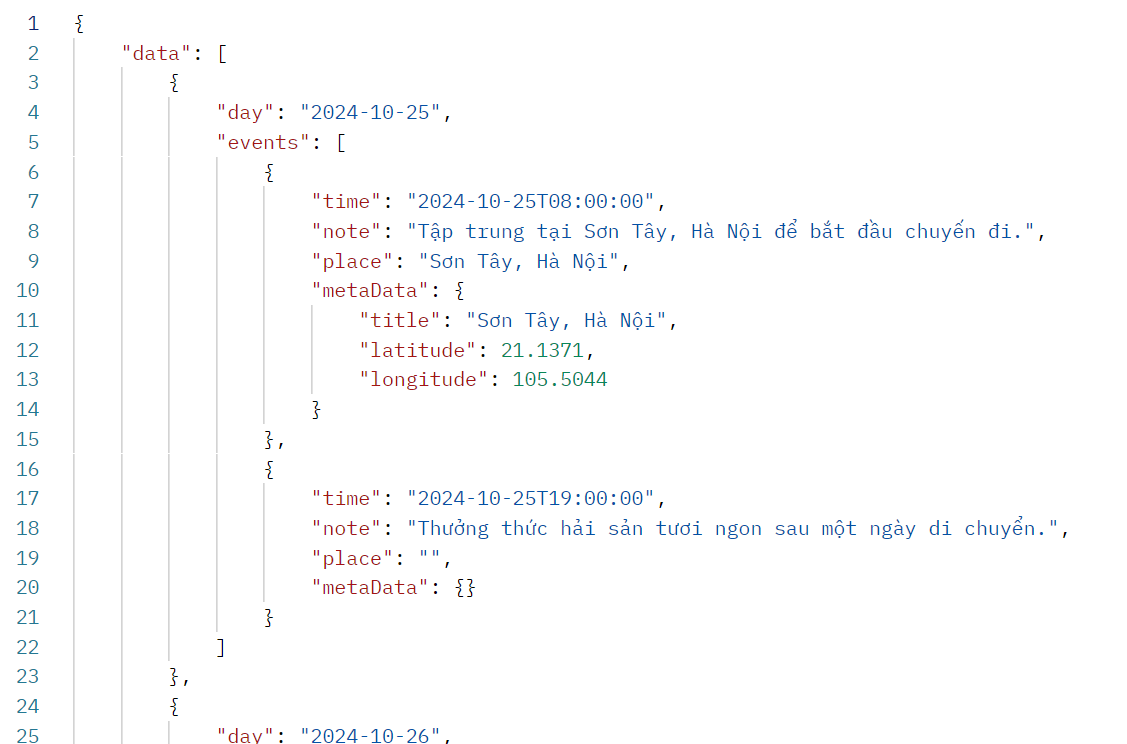
\includegraphics[width=1\textwidth]{figures/c4/output.png}
        \caption{Output JSON chứa lịch trình trả về từ server.}
        \label{fig:output}
    \end{figure}
\end{enumerate}

\noindent Kiến trúc xử lý hai giai đoạn này, kết hợp tiền xử lý bất đồng bộ và tổng hợp thông minh theo yêu cầu bằng LLM, cho phép VieVu cung cấp tính năng hỗ trợ tạo lịch trình mạnh mẽ và hiệu quả.